%vorlage%


\documentclass[12pt, captions=nooneline, titlepage, footsepline, headsepline]{scrartcl}
\usepackage[ngerman]{babel}
\usepackage{amsmath}
\usepackage{amssymb}
\usepackage{amsthm}
\usepackage{tabularx}
\usepackage{setspace} 
\usepackage{booktabs}
\usepackage{graphicx}
\usepackage{float}
\usepackage[a4paper,lmargin={2.5cm},rmargin={2.5cm},tmargin={2cm},bmargin={2cm}]{geometry}
\usepackage[backend=biber, style=alphabetic, citestyle=numeric]{biblatex}
\usepackage{csquotes}
\usepackage{helvet}
\addbibresource{literatur.bib}

%Kopf- und Fußzeile
\usepackage[automark]{scrlayer-scrpage} 
\pagestyle{scrheadings} 
\clearscrheadings 
\clearscrplain 
\rohead{\headmark} 
\lofoot{} 
\cofoot{} 
\rofoot{\pagemark}
\makeatletter
\usepackage{geometry}
\geometry{a4paper,
          left=25mm,right=25mm,top=20mm,bottom=20mm,
          includehead=false, % Kopfzeile außerhalb des Textkörper, also im Rand
          includefoot=false,
          headheight = \baselineskip,
          headsep = \dimexpr\Gm@tmargin-\headheight-10mm,
          footskip = \dimexpr\Gm@bmargin-10mm,
          %showframe,
          bindingoffset=0mm}
% Kopfzeile 1,0 cm Abstand zum Blattrand
% Fußzeile 1,0 cm Abstand zum Blattrand
\makeatother
\samepage
\linespread{1.3}
\newcommand\frontmatter{%
    \cleardoublepage
  %\@mainmatterfalse
  \pagenumbering{Roman}}

\newcommand\mainmatter{%
    \cleardoublepage
 % \@mainmattertrue
  \pagenumbering{arabic}}

\newcommand\backmatter{%
  \if@openright
    \cleardoublepage
  \else
    \clearpage
  \fi
 % \@mainmatterfalse
   }
   
\newcommand{\absatz}{\vspace{12pt}\noindent}
\newcommand{\logisch}[1]{$``#1``$}


%Dokument-Anfang
\begin{document}
% ! Bessere Übersicht fürs Ausfüllen der Daten

% * Titel der Arbeit
\newcommand{\var_titel_titel}{ewqewq}
% * Abgabedatum der Arbeit
\newcommand{\var_titel_datum}{ewqewq}

% * Autor 1
\newcommand{\var_titel_autor1}{ewqewq}
% * Autor 2
\newcommand{\var_titel_autor2}{weqewq}
% * Autor 3
\newcommand{\var_titel_autor3}{ewqewq}

% * Studiengang
\newcommand{\var_titel_studiengang}{qewewq}
% * Studienrichtung
\newcommand{\var_titel_studienrichtung}{ewqewq}
% * Seminargruppe
\newcommand{\var_titel_seminargruppe}{eqweqw}

% * Matrikelnummer 1
\newcommand{\var_titel_matrikel1}{eqwewq}
% * Matrikelnummer 2
\newcommand{\var_titel_matrikel2}{ewqewq}
% * Matrikelnummer 3
\newcommand{\var_titel_matrikel3}{ewqeqw}

% * Gutachter 1
\newcommand{\var_titel_gutachter1}{ewqewq}
% * Institut 1
\newcommand{\var_titel_institut1}{eqwewq}
% * Gutachter 2
\newcommand{\var_titel_gutachter2}{qewqewq}
% * Institut 2
\newcommand{\var_titel_institut2}{qwewqewq}

%Verzeichnis vorm Textteil
%Formelverzeichnis fehlt
\frontmatter
%Titelseite

\begin{titlepage}
\begin{center}

\textbf{\Huge Projektarbeit}\\
\vspace{1.5cm}
\LARGE{\vartiteltitel \\}
\vspace{1.5cm}
\end{center}
\begin{flushleft}
\large{
\begin{tabular}{l l r}
\vspace{1.0cm}
\textbf{Vorgelegt am:}\quad\quad\quad & \vartiteldatum\\

\textbf{Von:}           ~ & \textbf{\vartitelautor1}\\
                        ~ & \textbf{\vartitelautor2}\\
\vspace{1.0cm}
                        ~ & \textbf{\vartitelautor3}\\

\textbf{Studiengang:}   ~ & \vartitelstudiengang \\
\vspace{1.0cm}
\textbf{Studienrichtung:} ~ & \vartitelstudienrichtung \\
\vspace{1.0cm}
\textbf{Seminargruppe:} ~ & \vartitelseminargruppe \\

\textbf{Matrikelnummer:} ~ & \vartitelmatrikel1 \\
                         ~ & \vartitelmatrikel2 \\
\vspace{1.0cm}
                         ~ & \vartitelmatrikel3 \\
\textbf{Gutachter:}     ~ & \vartitelgutachter1 \\ ~ & (\vartitelinstitut1)\\
                        ~ & \vartitelgutachter2 \\ ~ & (\vartitelinstitut2)\\
                        
\end{tabular}}
\end{flushleft}
\end{titlepage}
\newpage
\newpage 
\thispagestyle{empty}
\quad  \addtocounter{page}{-1}
\newpage
\tableofcontents
\newpage
\addsec{Abbildungsverzeichnis}
\renewcommand\listfigurename{}
\listoffigures
\newpage
\addsec{Tabellenverzeichnis}
\renewcommand\listtablename{}
\listoftables

%Hauppteil geht hier los / Includes müssen hier dazu geschrieben werden / Pro Überkapitel ein Inklude
\mainmatter

%Alle Seiten beginnen mit der Oberüberschrift
\section{Einleitung}
Die ist eine PDF mit der Vorlage erstellt, um die Funktion und Formatierung dieser zu zeigen.
Deswegen wird in dieser Seite direkt ein Zitat\onlinezitat{LogikSim} verwendet.

\absatz Ganz wichtig zu wissen ist, dass \ac*{SSH} eine Abkürzung ist.

\absatz Ein Bild sollte außerdem nicht fehlen.
\bild[1.0]{schaltung1.png}{Ich bin ein tolles Bild}
\Blinddocument
%Kapitel groß endet mit:
\newpage
\section{Kapitel 2}
\subsection{Kapitel 2.1}

\newpage
\section{Kapitel 3
}

%Beispiel für eine Abbildung
\begin{figure}[H]
    \centering
    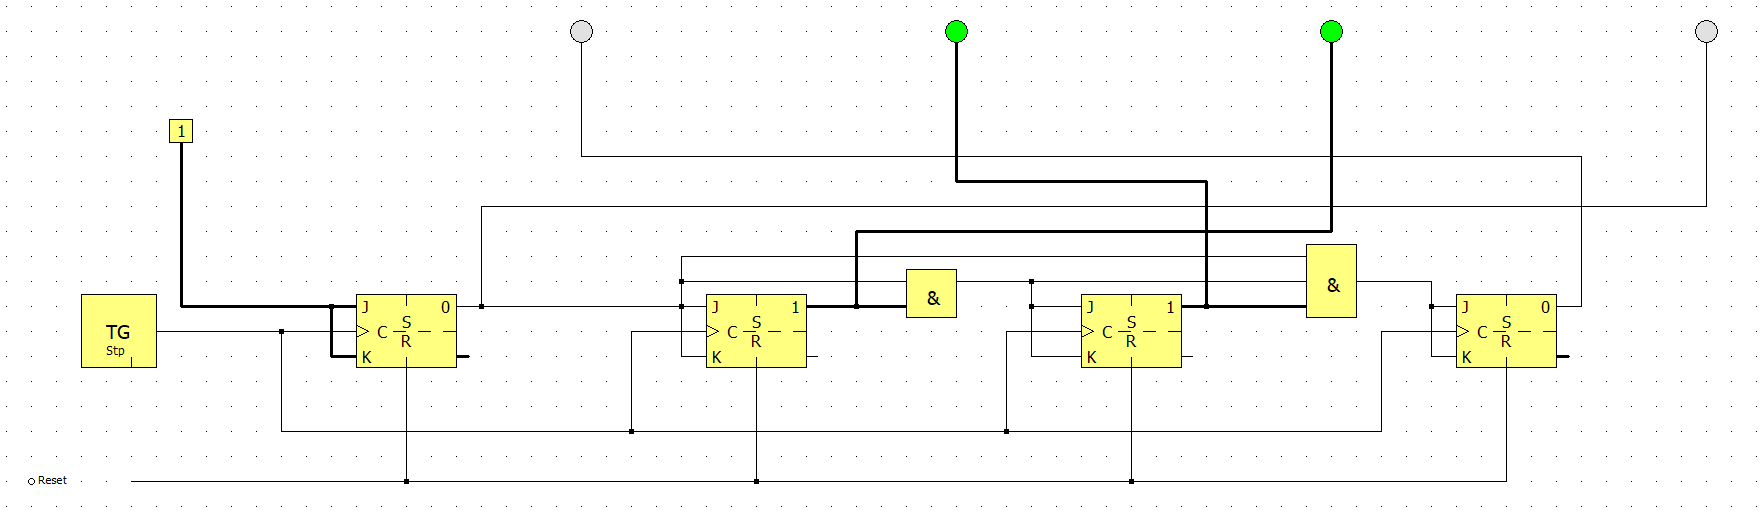
\includegraphics[width=1.0\columnwidth]{bilder/schaltung1.png}
    \caption{4-Bit synchroner Vorwärtszähler}
    \label{fig:4-Bit synchroner Vorwärtszähler}
\end{figure}


\newpage
\section{Kapitel 4}
\subsection{Kapitel 4.1}

\subsection{Kapitel 4.2}

\subsection{Kapitel 4.3}
\newpage
\section{Fazit}


\newpage

%Anhang
%Überschrift Anhang fehlt noch.
\addsec{Quellen- und Literaturverzeichnis}

%Literaturverzeichnis muss noch formatiert werden
\printbibliography
%!	Anhang

\clearpage
\appendix
\clearpage

%! Section Befehl wird umgeschrieben, damit keine Überschriften mehr angezeigt werden
%!Kann falls Überschriften gewollt sind entfern werden oder erst später eingefügt
% Beginn 
\renewcommand{\section}[1]{
\par\refstepcounter{section}
\sectionmark{#1}
\addcontentsline{atoc}{section}{\protect\numberline{\thesection}#1}
\lohead{\textnormal{#1}}
} % Ende

%! Hier kann man sich anpassen, wie Abbildungen im Anhang dargestellt werden.
%! Bitte eins der beiden Auskommentieren
%? Möglichkeit 1 ohne Nummerierung und ohne Abbildung davor 
%\renewcommand{\bild}[3][1.0]{\begin{figure}[H]
%	\centering
%	\includegraphics[width=#1\columnwidth]{bilder/#2}
%	\caption*{#3}
%	\label{fig:#3}
%	\end{figure}}

%? Möglichkeit 2 mit Nummerierung und Abbildung, aber nicht im Abbildungsverzeichnis
\renewcommand{\bild}[3][1.0]{\begin{figure}[H]
	\centering
	\includegraphics[width=#1\columnwidth]{bilder/#2}
	\caption[]{#3}
	\label{fig:#3}
	\end{figure}}

%! Anhang 1
\section{Erster toller Anhang}
Hihi hier kommt eigentlich ein Anhangverzeichnis hin :D
\clearpage

%! Anhang 2
\section{Inhalt der CD}
CD mit folgenden Inhalten:
\begin{itemize}
	\item dieses Dokument
	\item Latex Dateien
	\item Youtube-Video als Bonus
\end{itemize}
 \clearpage

%! Eidestattliche Erklärung, hier zwischen Version für einen oder mehrere Autoren umschalten
\input{inhalt/Erklärung_Praxisbeleg}
%\input{inhalt/Erklärung_3Autoren}

\include{Erklärung}
\end{document}
